\documentclass[compress]{beamer}
\usepackage[ngerman]{babel}
\usepackage{graphicx}
\usepackage{subfiles}
\usepackage{listings}

\graphicspath{{images/}}

% \setbeameroption{show notes}

\usetheme[noflama]{custom}

\title{Virtualisierte Arbeitsumgebung für den Test verteilter Systeme}
\subtitle{Microservice-Architektur mit Docker, Kafka, Clojure \& Elm}
\author{Jan-Philipp Willem}
\institute{Fakultät für Informatik\\Hochschule Mannheim}
\date{21. Juni 2017}

\begin{document}

% \begin{frame}[noframenumbering,plain]
% \end{frame}

\maketitle

% \begin{frame}[noframenumbering,plain]{Project-Repository}
  % \includegraphics[width=0.8\textwidth]{google.pdf}
% \end{frame}

\section*{Gliederung}
\begin{frame}[noframenumbering,plain]{Gliederung}
  \tableofcontents[hideallsubsections]
\end{frame}

\section{Kontext}
\begin{frame}{Bisheriger Ablauf}
\end{frame}
\begin{frame}{Anforderungen}
\end{frame}
\begin{frame}{Erhoffte Vorteile}
\end{frame}

\section{Docker}
\begin{frame}{Description}
\end{frame}
\begin{frame}{Container}
\end{frame}
\begin{frame}{Docker-Compose}
\end{frame}

\section{Inspiration}
\begin{frame}{Tmux Panes}
  
  % \AddToShipoutPictureFG*{%
    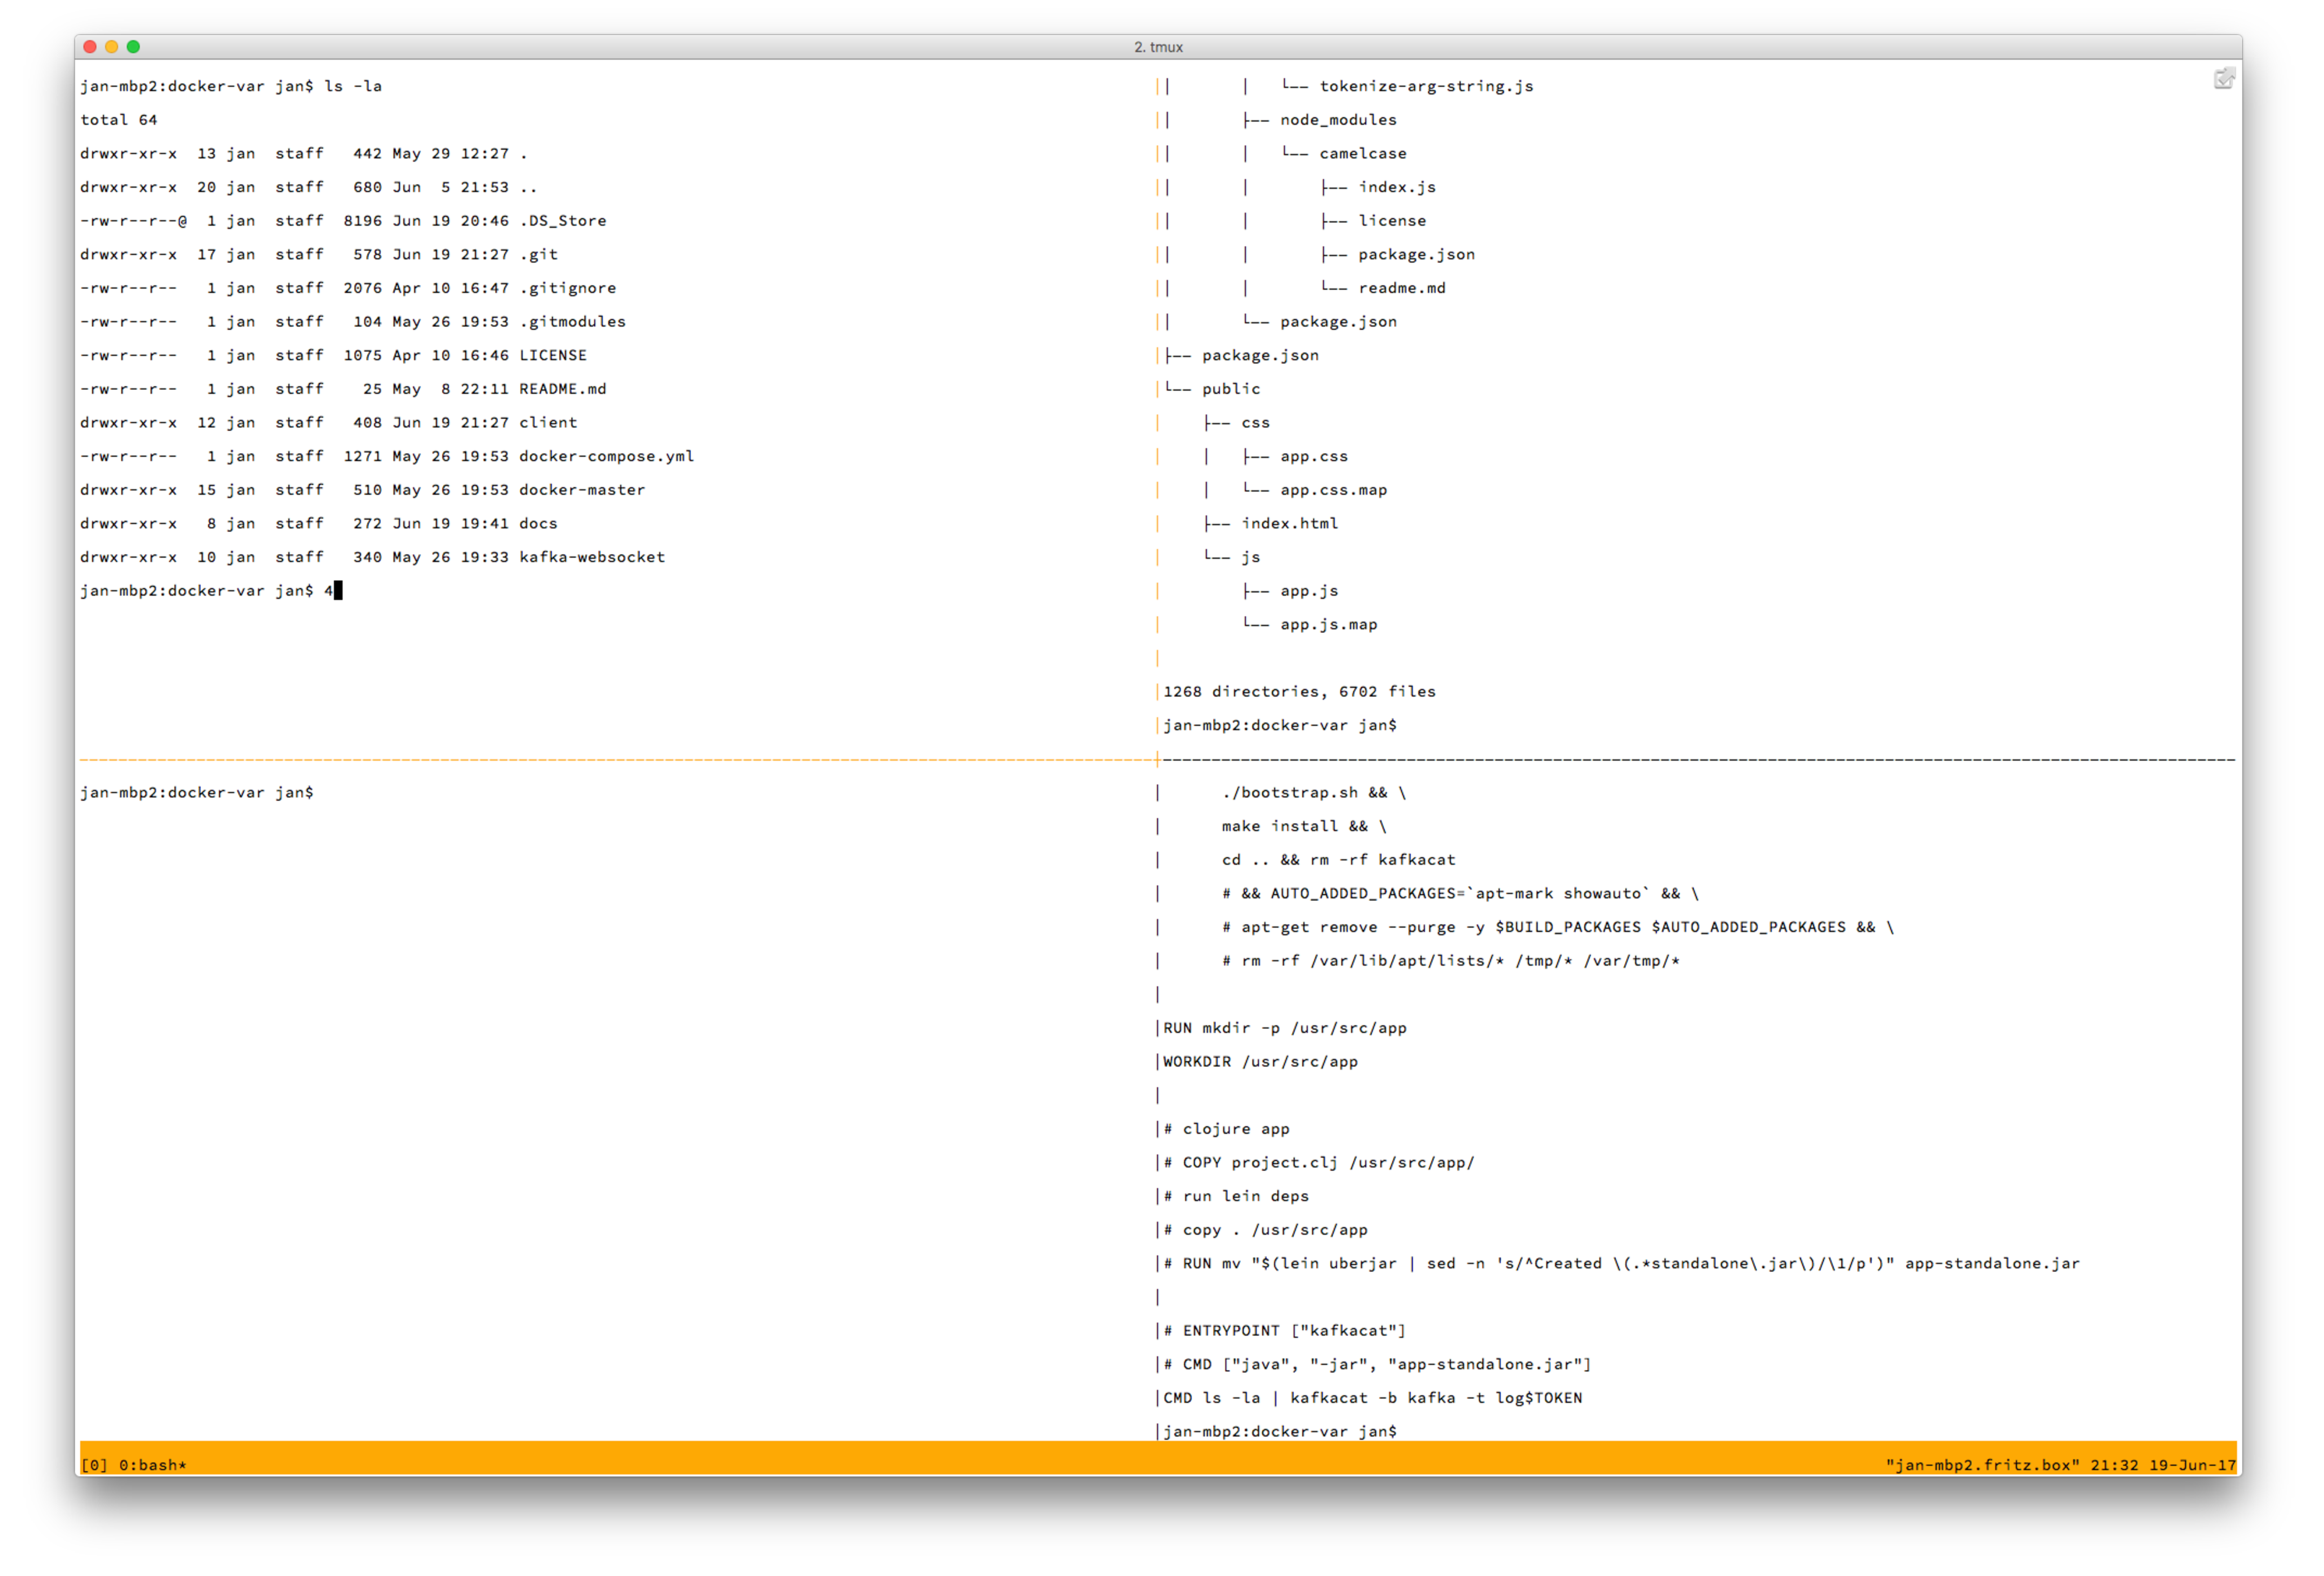
\includegraphics[width=\textwidth]{tmux.pdf}
  % }
\end{frame}
\begin{frame}{Cloud-IDEs}
\end{frame}
\begin{frame}{xterm.js}
  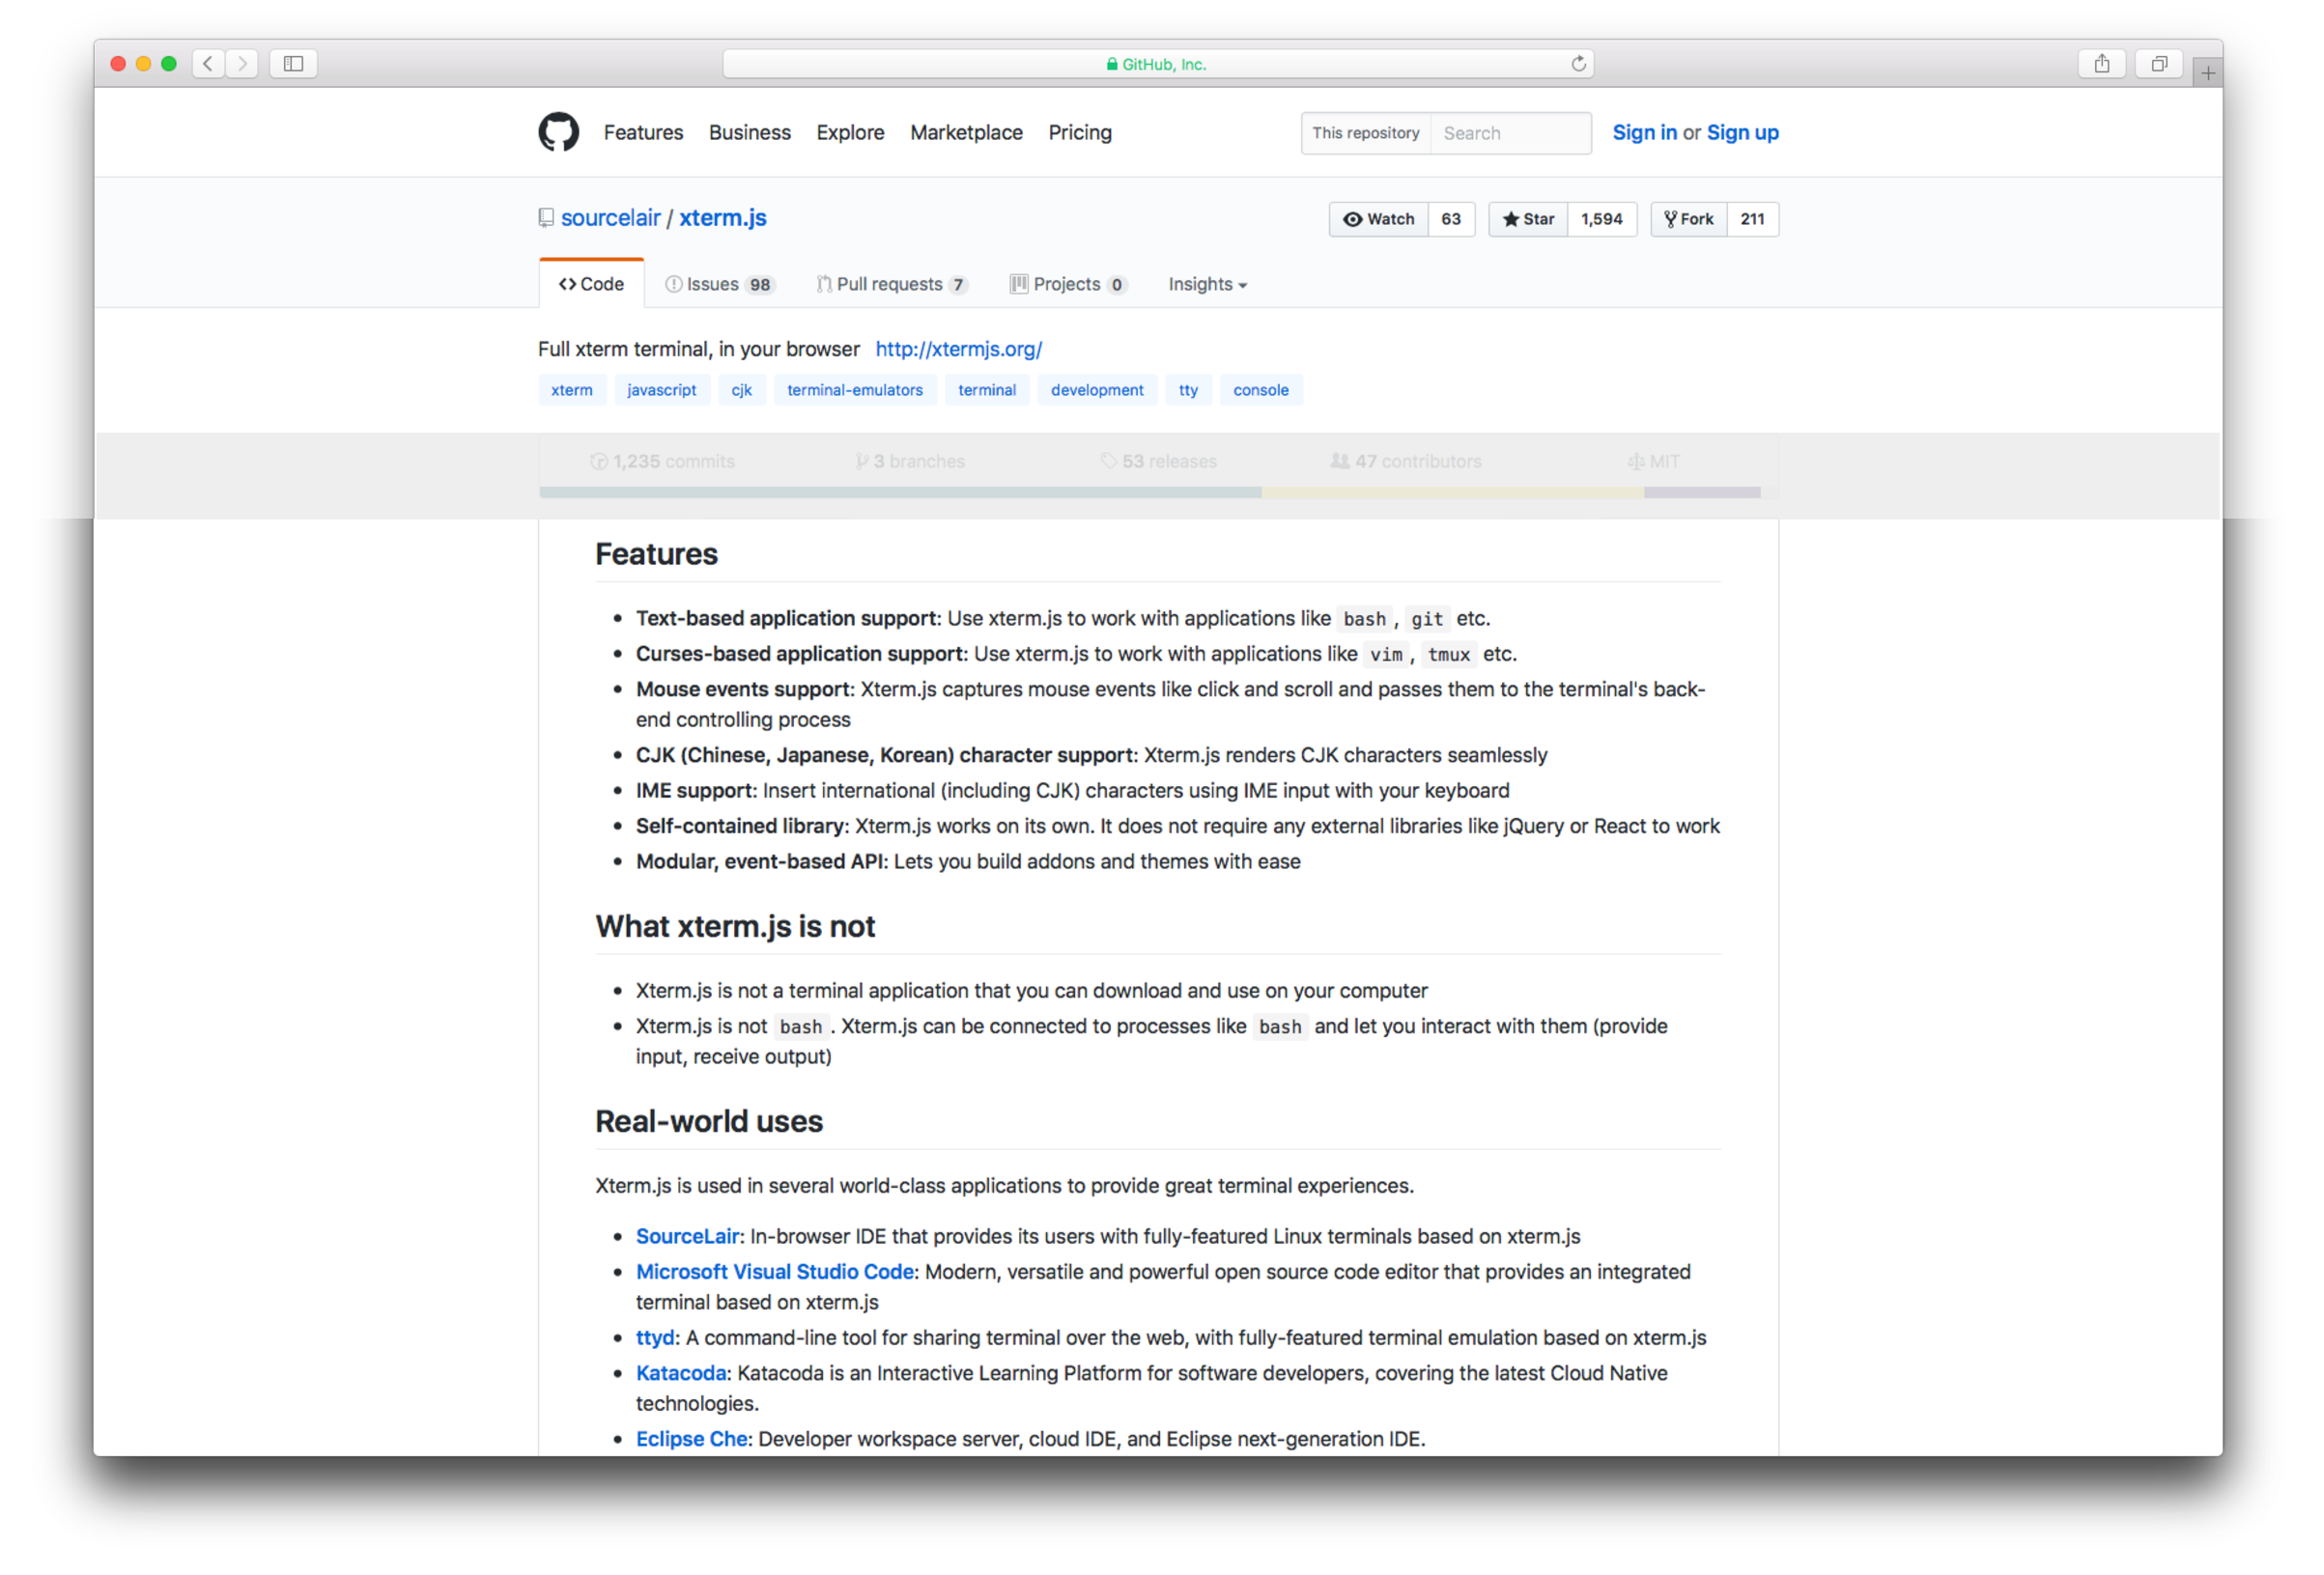
\includegraphics[width=\textwidth]{xterm.pdf}
\end{frame}
\begin{frame}{ttyd}
  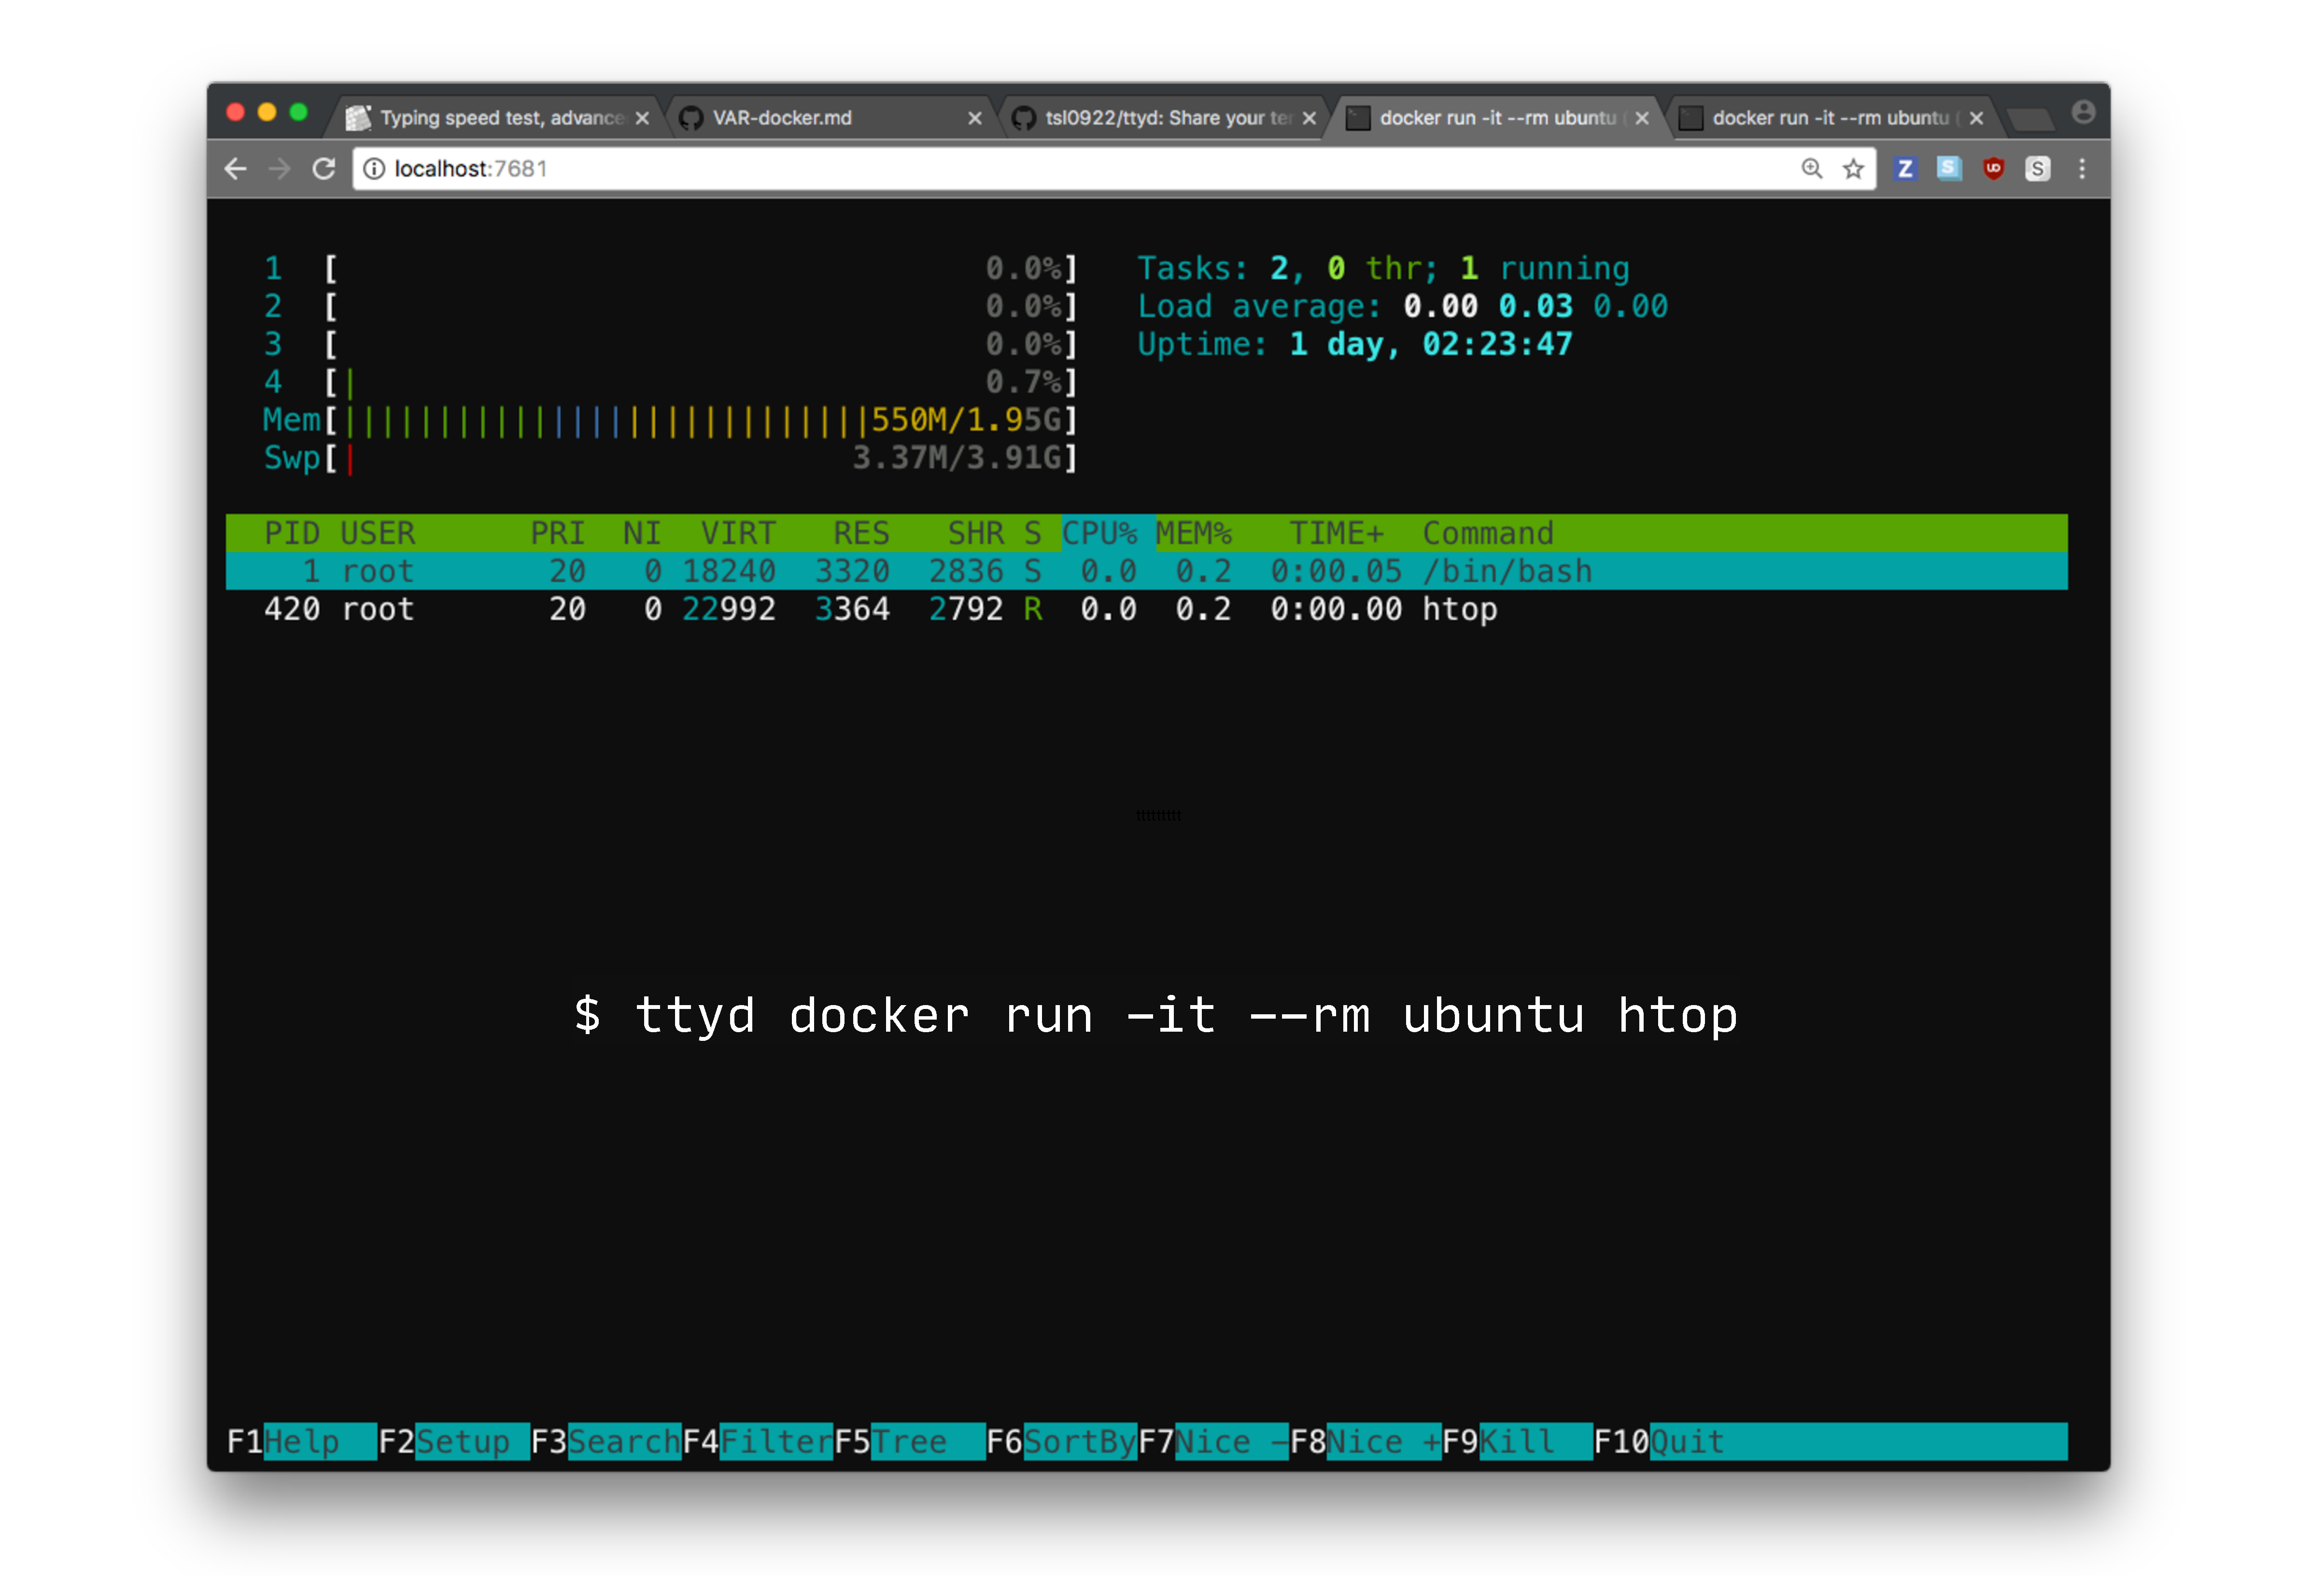
\includegraphics[width=\textwidth]{ttyd.pdf}
\end{frame}

\section{„VAR-Tool“}
\begin{frame}{}
  \AddToShipoutPictureFG*{%
    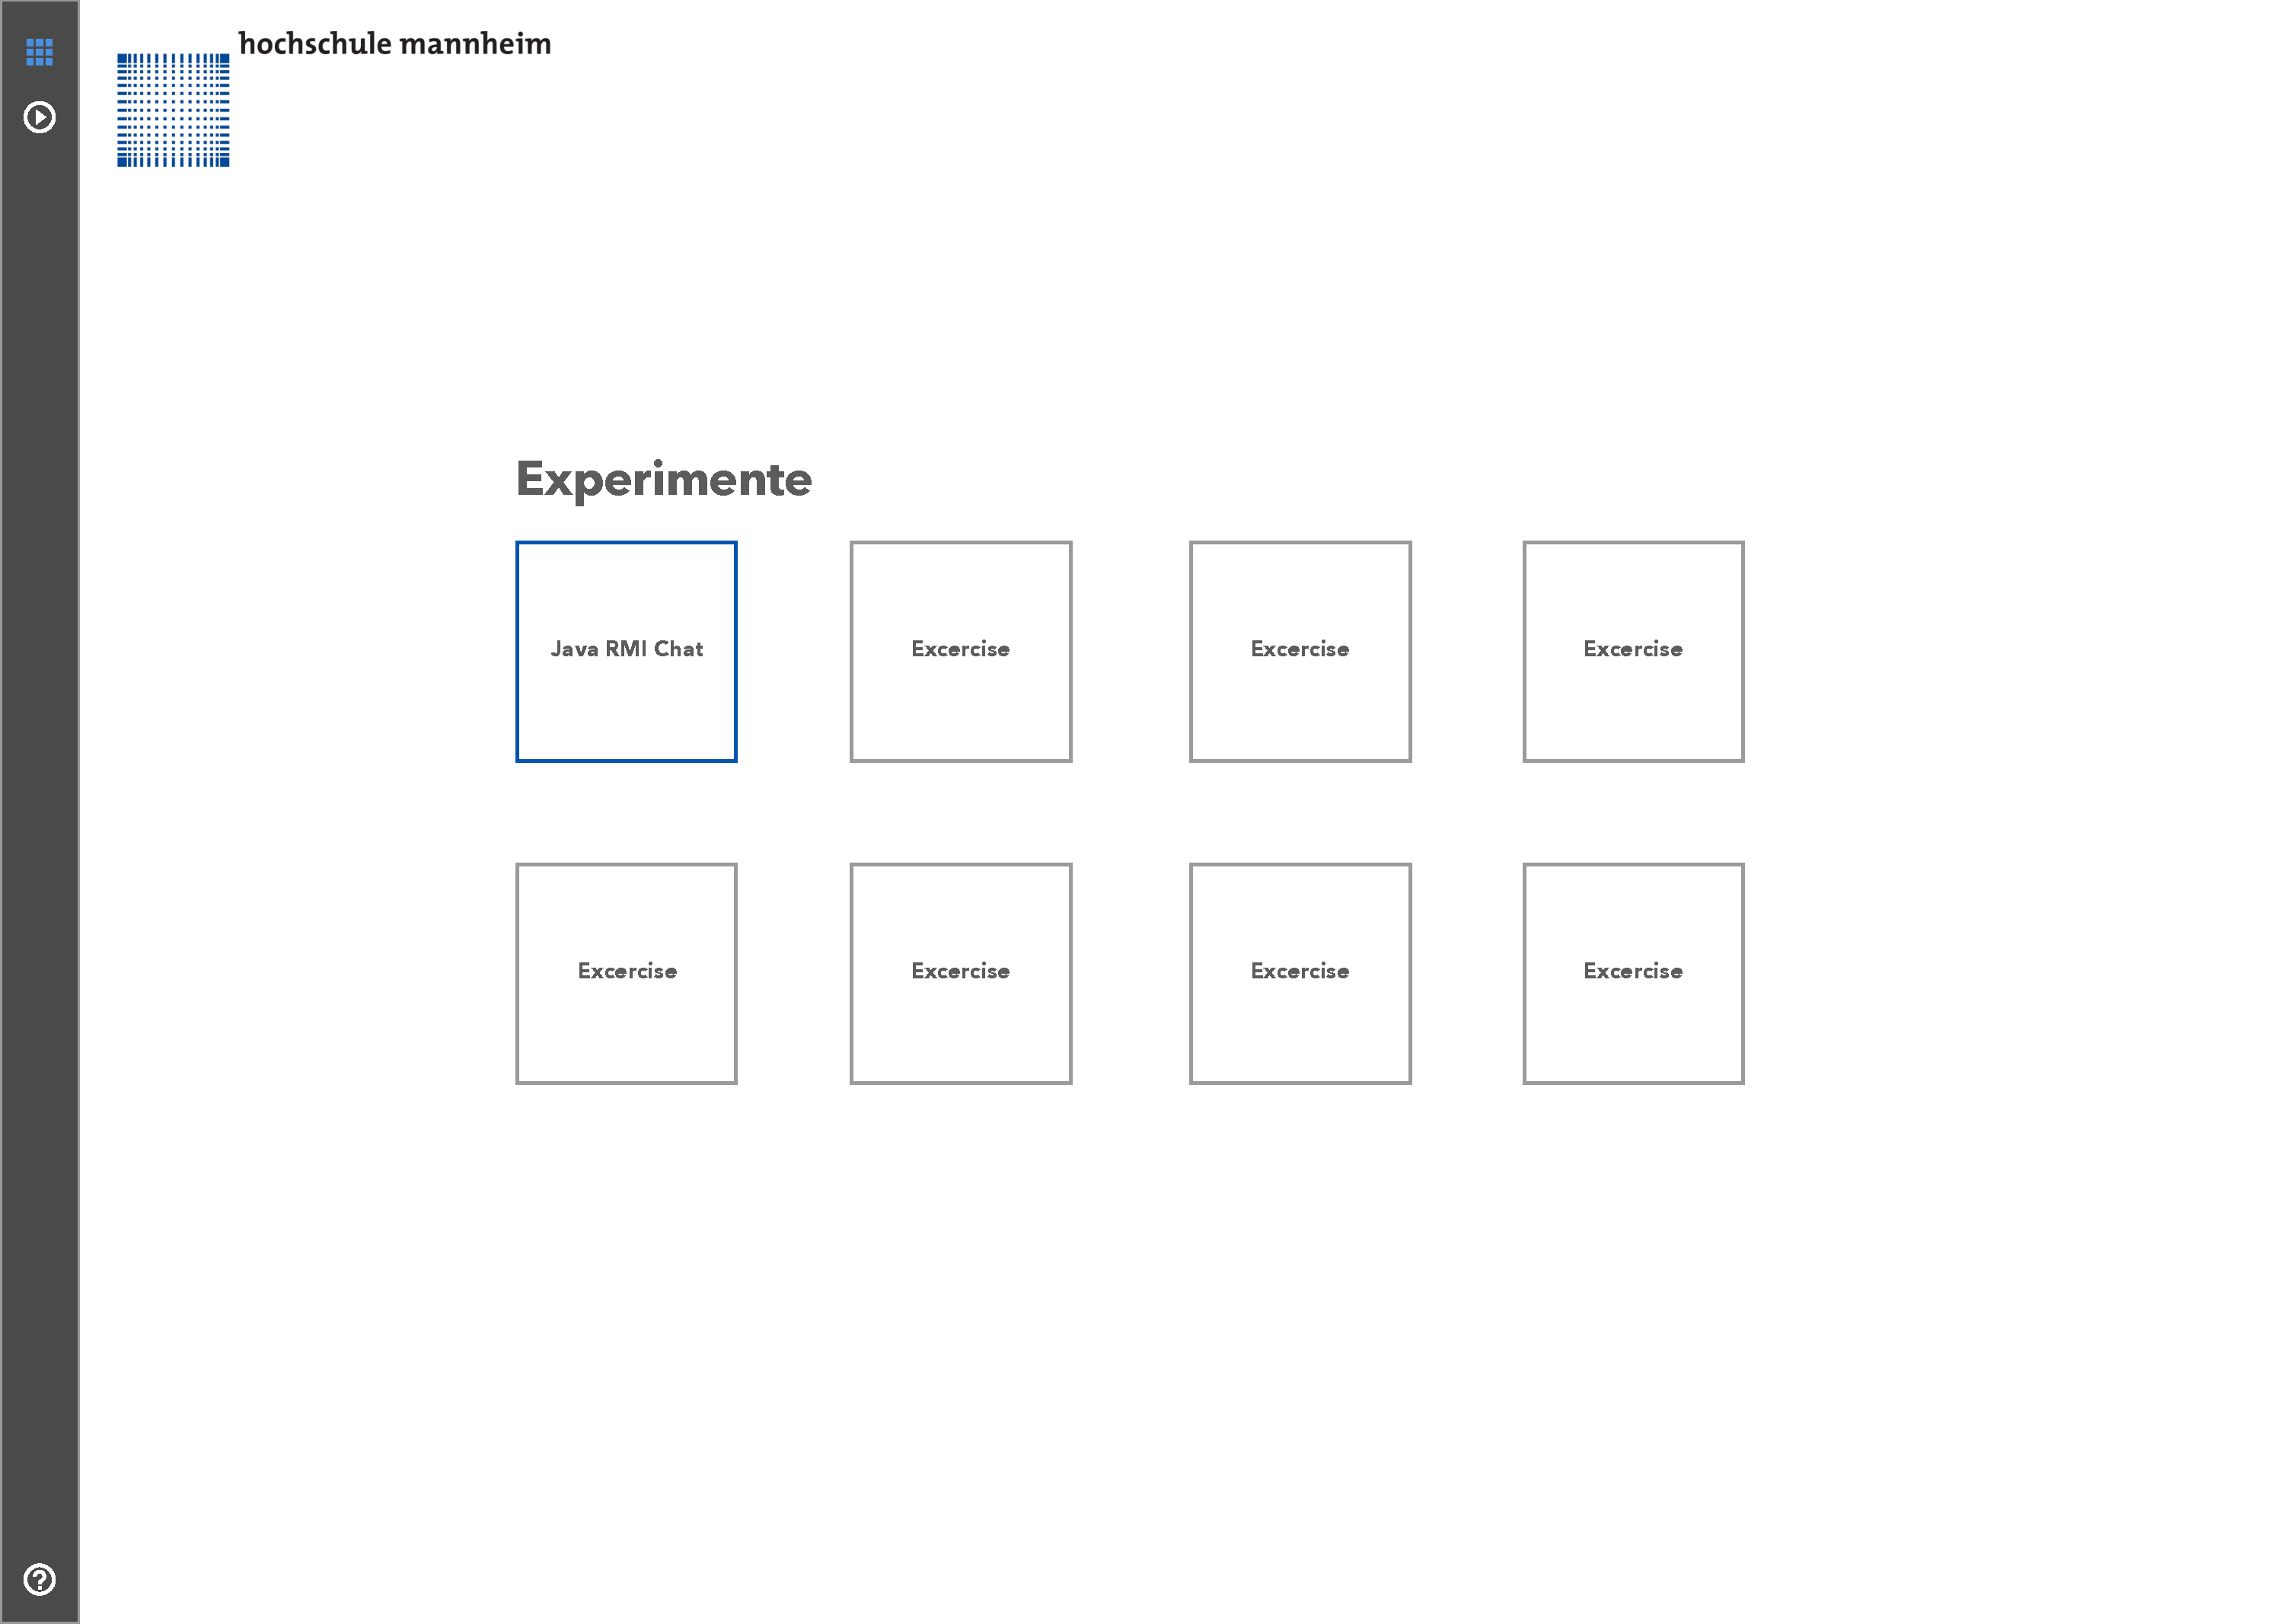
\includegraphics[width=\paperwidth,height=\paperheight,page=1]{ui-mockup.pdf}
  }
\end{frame}
\begin{frame}{}
  \AddToShipoutPictureFG*{%
    \includegraphics[width=\paperwidth,height=\paperheight,page=2]{ui-mockup.pdf}
  }
\end{frame}
\begin{frame}{Network}
  \AddToShipoutPictureFG*{%
    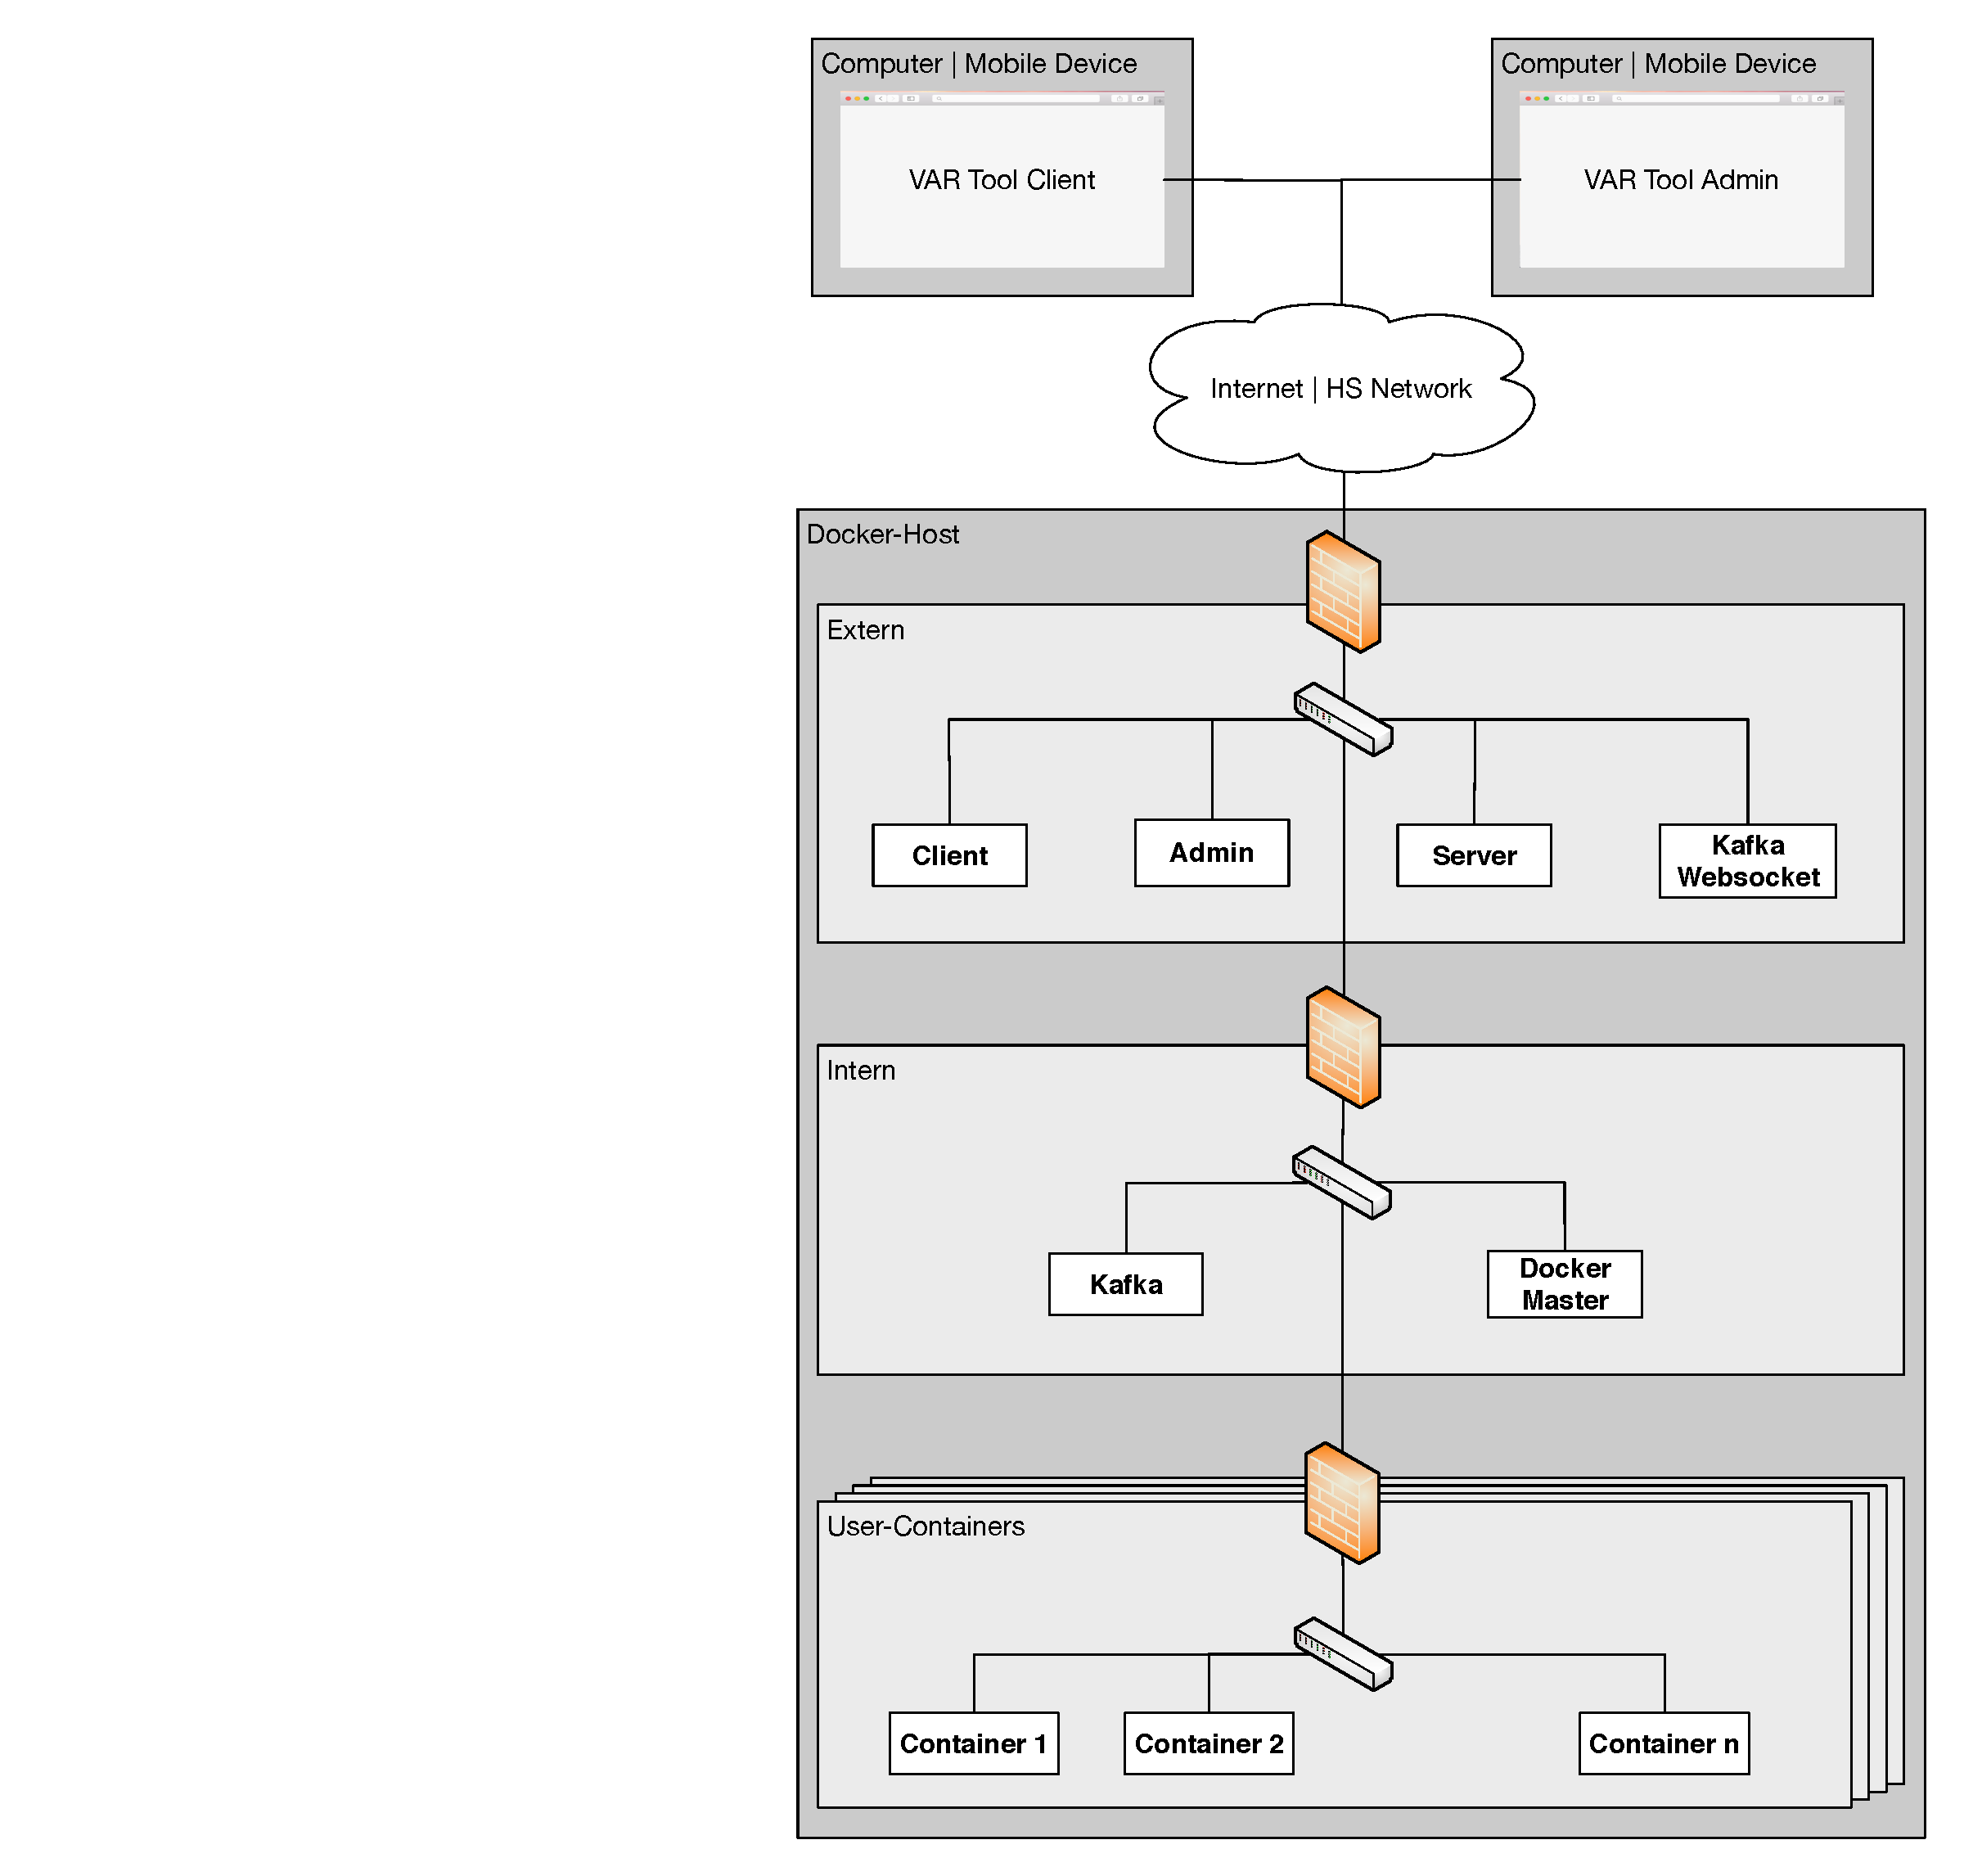
\includegraphics[height=\textheight]{network.pdf}
  }
\end{frame}
\begin{frame}{Sequence}
  \AddToShipoutPictureFG*{%
    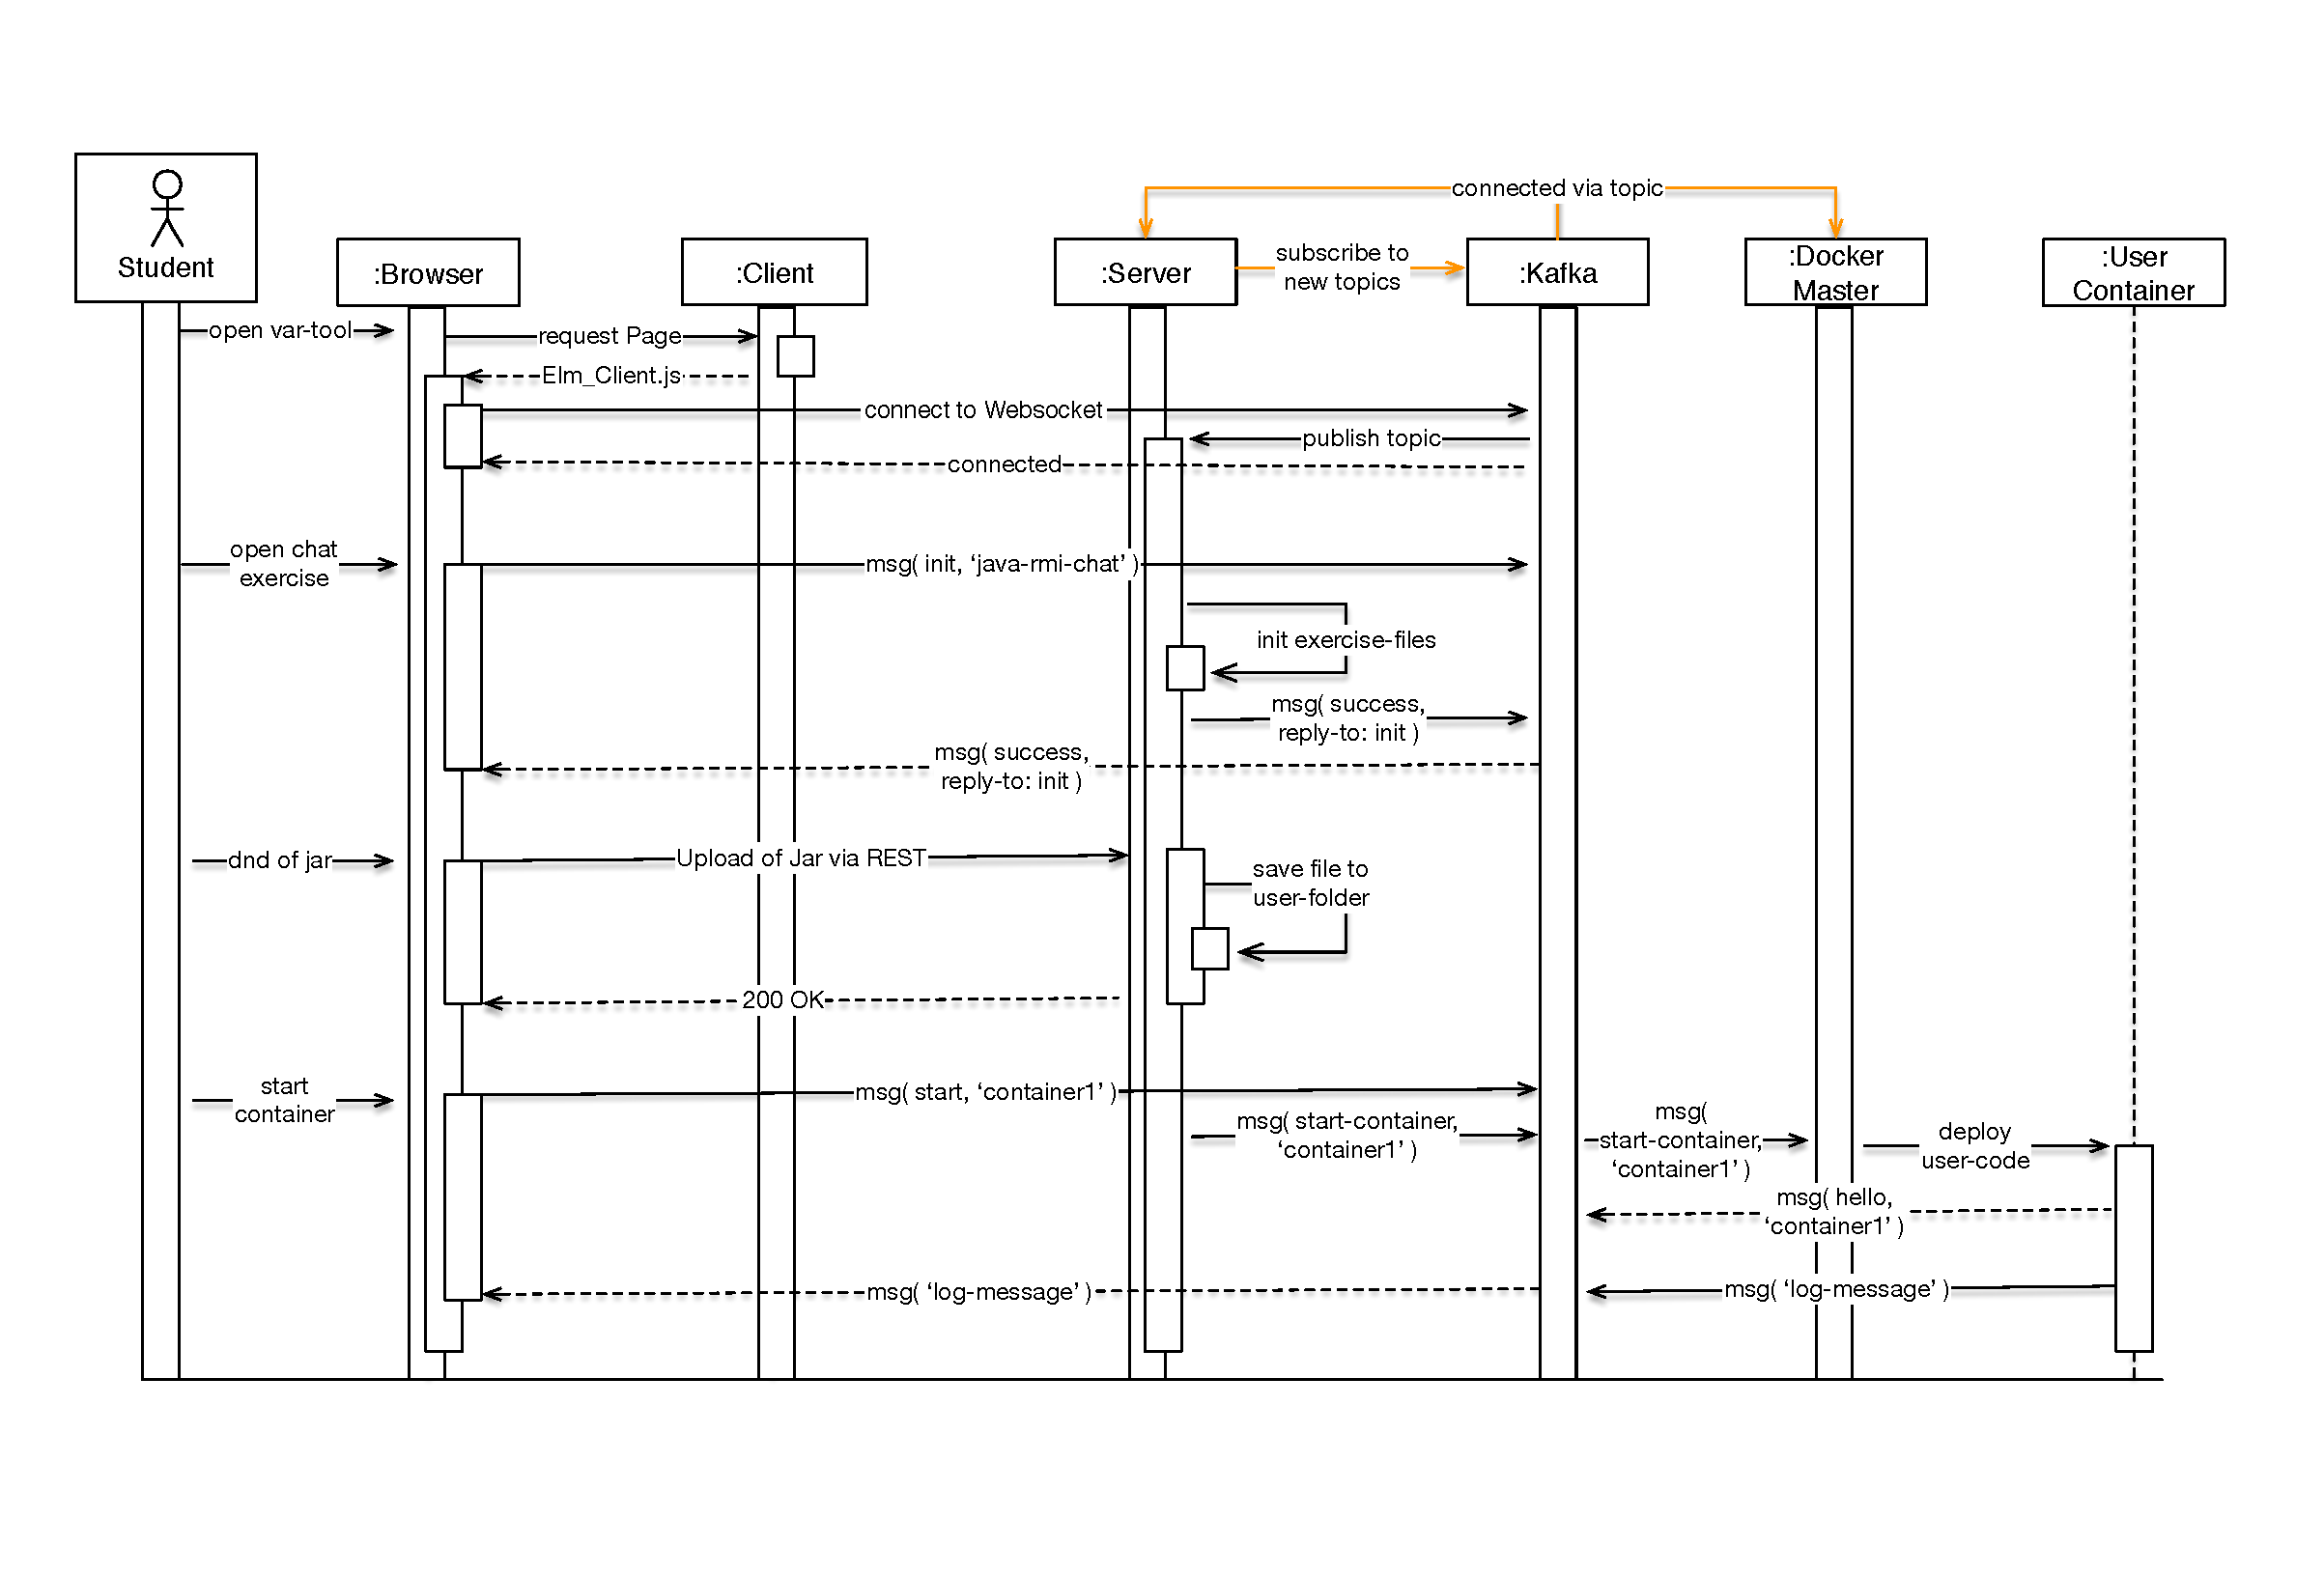
\includegraphics[height=\textheight]{sequence.pdf}
  }
\end{frame}
\begin{frame}[noframenumbering,plain]{Deployment}
  \AddToShipoutPictureFG*{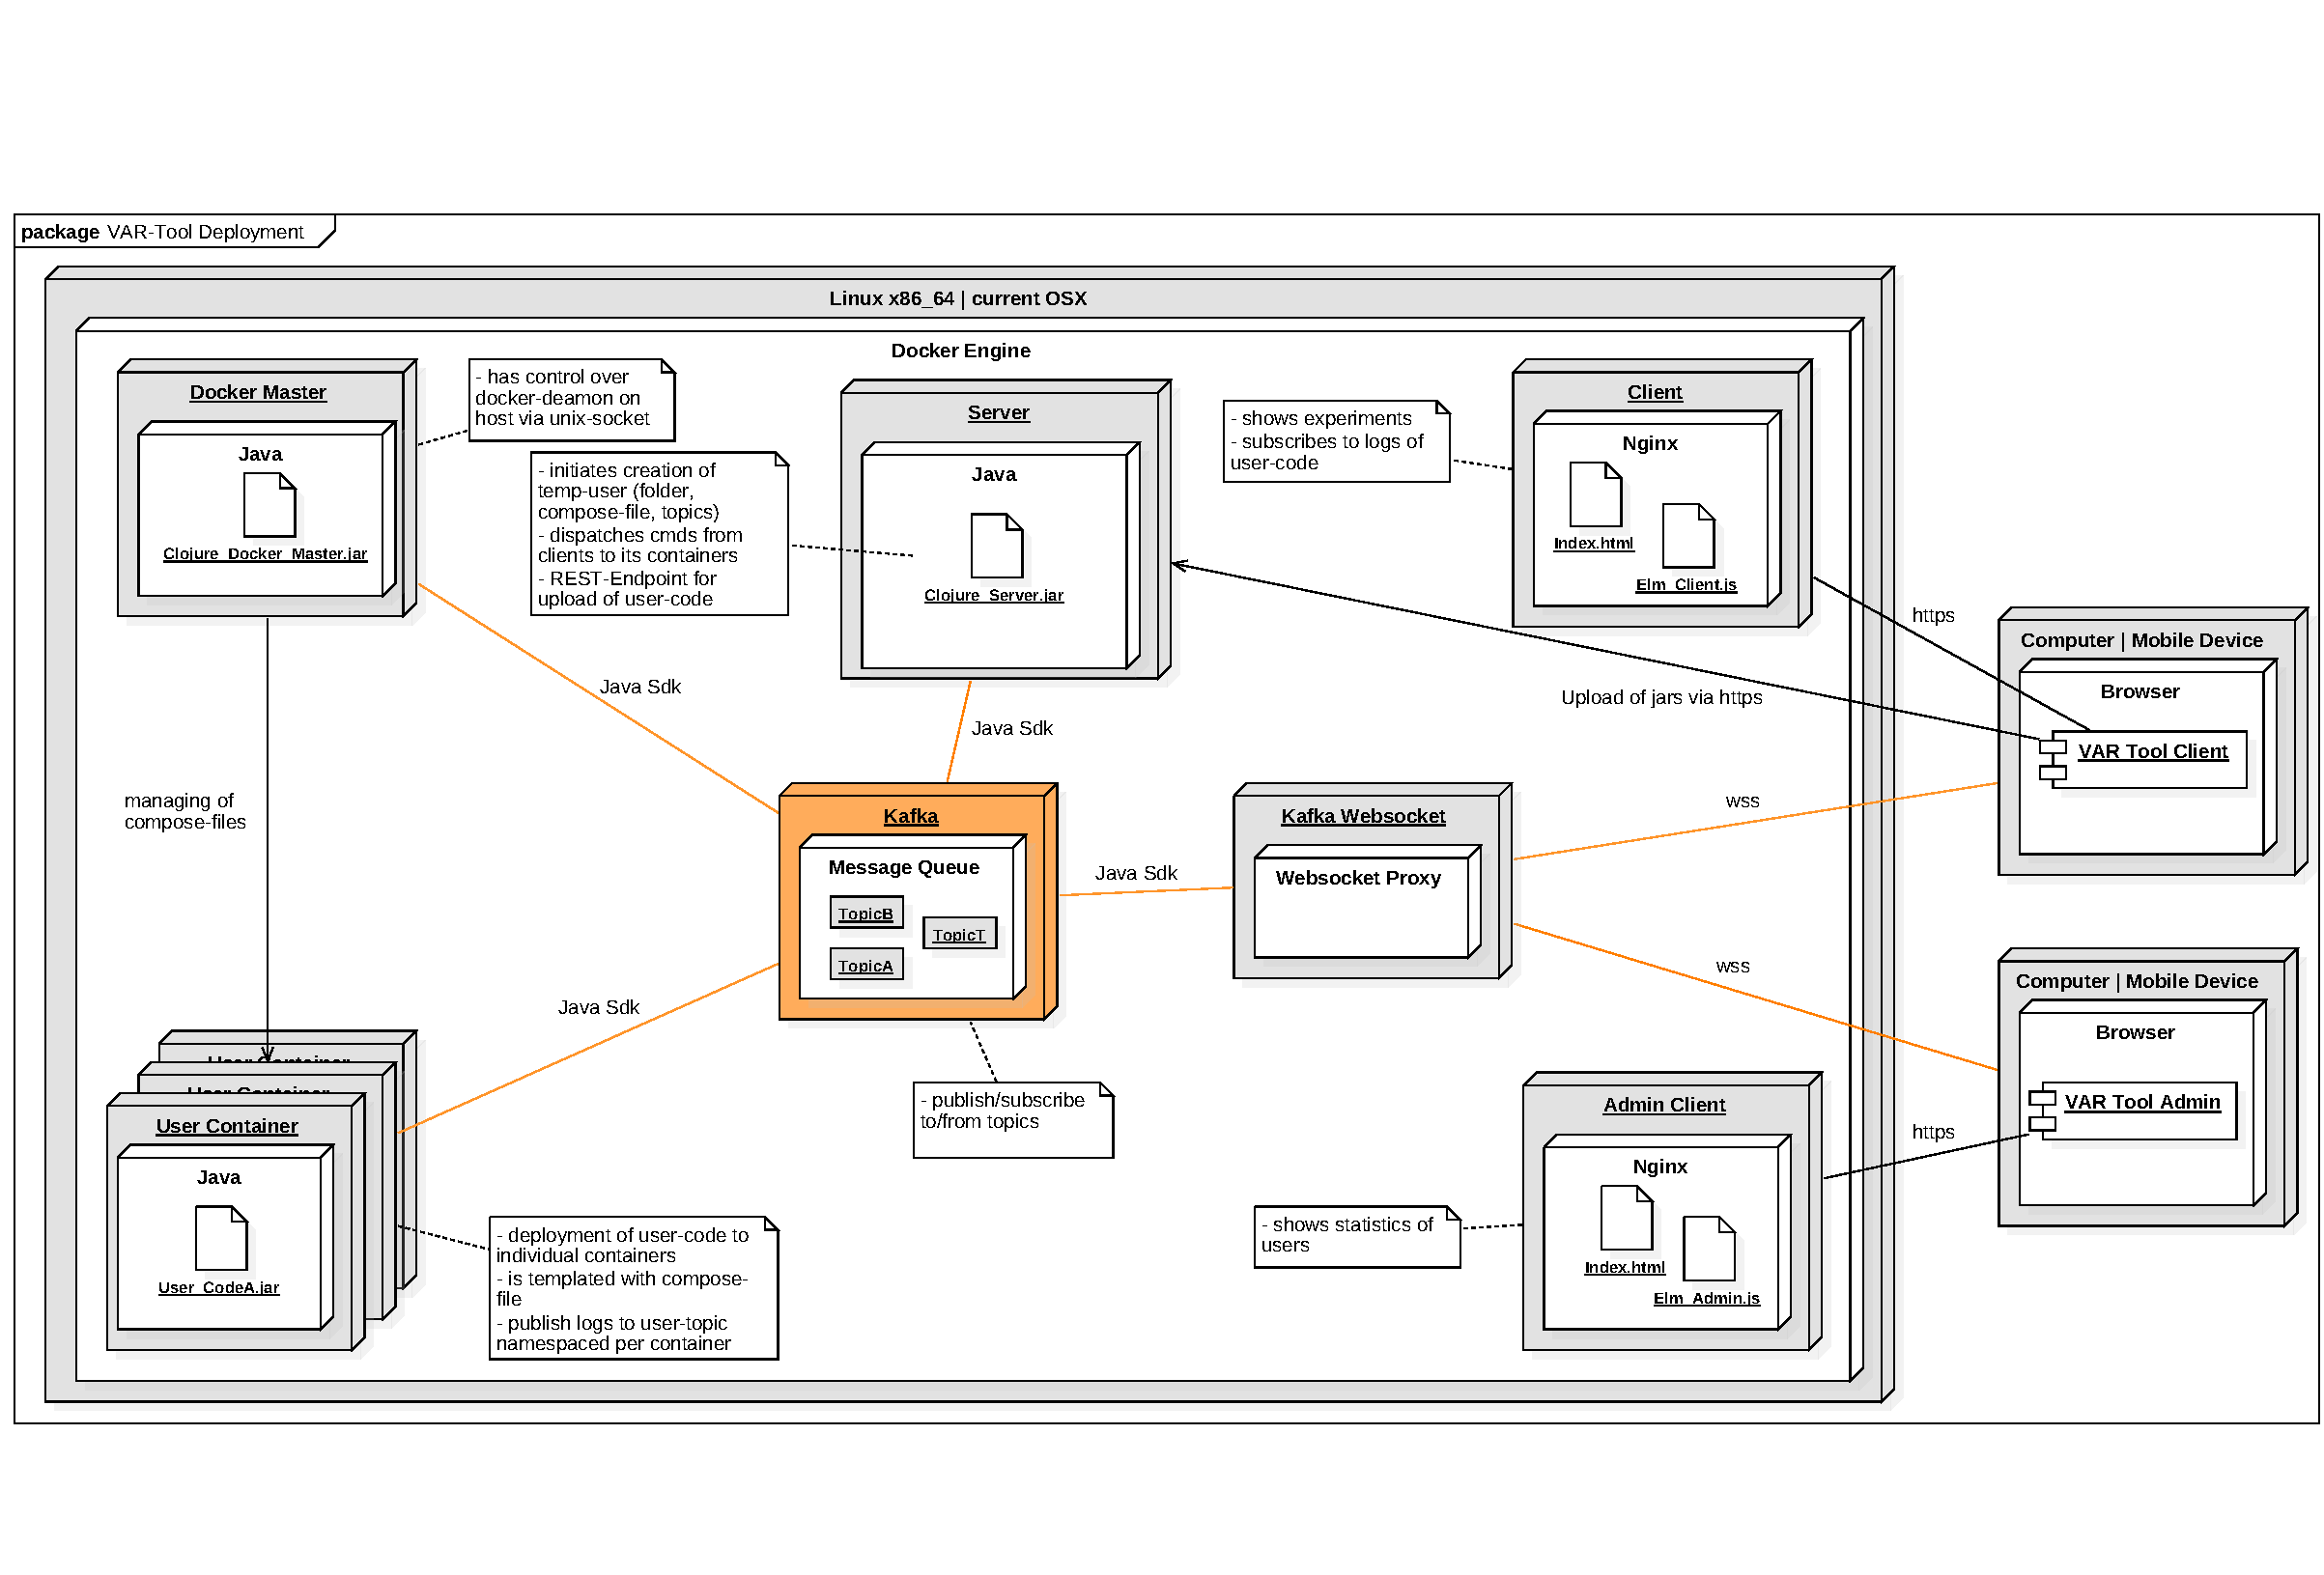
\includegraphics[width=\paperwidth]{deployment.pdf}}
\end{frame}
\begin{frame}{Compose-File}
\end{frame}

\section{Ausblick}
\begin{frame}{Ausblick}
\end{frame}

\begin{frame}[noframenumbering,plain]{Fin}
  Danke für die Aufmerksamkeit. -- Fragen?
\end{frame}
\end{document}
